\section{Results and Analysis}

\subsection{Main Results}

Table~\ref{tab:main-results} summarizes SAQT results on MTHv2 and HDRC. All results use dataset-level micro AR/CR. \emph{Direct} denotes greedy CTC decoding without logit bias. \emph{Calibrated} denotes blank/nonblank logit bias determined on the development split and fixed for testing.

\begin{table}[t]
\centering
\caption{SAQT test results on MTHv2 and HDRC.}
\label{tab:main-results}
\begin{tabular}{llrrrr}
\toprule
Dataset & Decode & Bias & Samples & AR & CR \\
\midrule
MTHv2 & Direct & 0/0 & 10455 & 96.33 & 96.50 \\
MTHv2 & Calibrated & -2.0/0.8 & 10455 & 96.75 & 97.00 \\
HDRC & Direct & 0/0 & 3381 & 91.50 & 91.64 \\
HDRC & Calibrated & -2.0/1.0 & 3381 & 93.44 & 94.36 \\
\bottomrule
\end{tabular}
\end{table}

Under direct decoding, SAQT obtains AR/CR of 96.33/96.50 on MTHv2 and 91.50/91.64 on HDRC. With the development-set-fixed blank/nonblank bias, the results become 96.75/97.00 and 93.44/94.36, respectively. We report both settings because direct decoding shows the uncalibrated CTC recognizer, while calibrated decoding follows a fixed protocol for adjusting a global blank/nonblank bias before test evaluation.

\subsection{Comparison with Adapted Scene Text Recognizers}

Table~\ref{tab:baseline-comparison} compares SAQT with scene text recognizers adapted to vertical input. To avoid protocol mismatch, all baseline predictions are converted to the same micro AR/CR metrics.

\begin{table}[t]
\centering
\caption{Comparison with vertical-input-adapted scene text recognizers.}
\label{tab:baseline-comparison}
\begin{tabular}{llrr}
\toprule
Dataset & Model & AR & CR \\
\midrule
MTHv2 & CRNN & 95.51 & 95.63 \\
MTHv2 & SVTR-tiny & 95.56 & 95.68 \\
MTHv2 & SVTR-small & 95.34 & 95.44 \\
MTHv2 & SVTR-L & 95.16 & 95.26 \\
MTHv2 & ABINet & 90.75 & 90.91 \\
MTHv2 & SAR & 73.20 & 87.65 \\
\midrule
HDRC & CRNN & 84.91 & 85.21 \\
HDRC & SVTR-tiny & 83.71 & 83.89 \\
HDRC & SVTR-L & 78.16 & 78.43 \\
HDRC & ABINet & 77.61 & 77.84 \\
HDRC & SAR & 70.74 & 73.24 \\
\bottomrule
\end{tabular}
\end{table}

On MTHv2, SAQT under direct decoding achieves 96.33/96.50 AR/CR, which is higher than the closest adapted baseline, SVTR-tiny, at 95.56/95.68. With the fixed calibration protocol, SAQT reaches 96.75/97.00. On HDRC, SAQT under direct decoding achieves 91.50/91.64, compared with 84.91/85.21 from the closest CRNN baseline. Calibration further changes SAQT to 93.44/94.36. Fig.~\ref{fig:main-results} visualizes the same comparison. These results indicate that the overall SAQT framework obtains higher AR/CR within the unified comparison protocol. The independent contribution of each training module should be separated by ablations, while calibration remains a lightweight inference-stage supplement.

\begin{figure}[t]
  \centering
  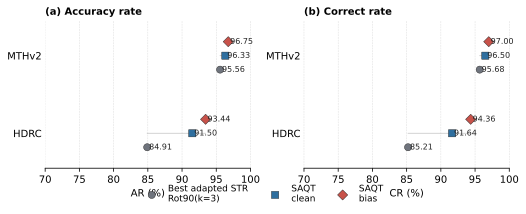
\includegraphics[width=\linewidth]{figures/figure2_main_results.pdf}
  \caption{Main comparison on MTHv2 and HDRC. The best adapted STR baseline is SVTR-tiny on MTHv2 and CRNN on HDRC.}
  \label{fig:main-results}
\end{figure}

\subsection{Effect of Query Activation Budget}

Table~\ref{tab:qbudget} evaluates the query activation budget on MTHv2. Both settings are evaluated on the same test set with the same AR/CR protocol.

\begin{table}[t]
\centering
\caption{Effect of query activation budget on MTHv2.}
\label{tab:qbudget}
\begin{tabular}{llrrrr}
\toprule
Setting & Decode & Bias & Samples & AR & CR \\
\midrule
w/o query budget & Direct & 0/0 & 10455 & 95.53 & 95.71 \\
w/o query budget & Calibrated & -2.0/1.0 & 10455 & 96.10 & 96.37 \\
w/ query budget & Direct & 0/0 & 10455 & 96.17 & 96.29 \\
w/ query budget & Calibrated & -2.0/0.8 & 10455 & 96.69 & 96.90 \\
\bottomrule
\end{tabular}
\end{table}

Under direct decoding, the query budget improves AR/CR from 95.53/95.71 to 96.17/96.29. With calibration, AR/CR improves from 96.10/96.37 to 96.69/96.90. This result supports the role of the length-aware activation constraint on MTHv2.

We further evaluate a qbudget-localization-query variant on HDRC in Table~\ref{tab:hdrc-qbudget-variant}, using the same downstream head reconstruction, full-model recognition training, and development-set calibration protocol as the HDRC mainline. This setting contains both the query-budget constraint and a different localization-aware query representation, and should therefore be interpreted as a variant-level comparison rather than a single-factor causal ablation.

\begin{table}[t]
\centering
\caption{HDRC qbudget-localization-query variant.}
\label{tab:hdrc-qbudget-variant}
\begin{tabular}{llrrrr}
\toprule
Variant & Decode & Bias & Samples & AR & CR \\
\midrule
mainline & Direct & 0/0 & 3381 & 89.99 & 90.33 \\
mainline & Calibrated & -2.0/0.4 & 3381 & 90.70 & 91.80 \\
qbudget-localization-query & Direct & 0/0 & 3381 & 91.50 & 91.64 \\
qbudget-localization-query & Calibrated & -2.0/1.0 & 3381 & 93.44 & 94.36 \\
\bottomrule
\end{tabular}
\end{table}

On HDRC, the qbudget-localization-query variant reaches 91.50/91.64 AR/CR under direct decoding and 93.44/94.36 after fixed calibration, higher than the corresponding mainline results. This provides additional target-domain evidence for the combined localization-aware query representation and activation-budget design, while keeping the claim strength limited to this variant comparison.

\subsection{Effect of the Length-Consistency Auxiliary Term}

Table~\ref{tab:expected-count} compares the MTHv2 results with and without the CTC expected-count auxiliary term. Both settings use the same query-budget branch and the same test protocol; the only difference is whether the length-consistency auxiliary term is added during recognition training.

\begin{table}[t]
\centering
\caption{Effect of the expected-count auxiliary term on MTHv2.}
\label{tab:expected-count}
\begin{tabular}{llrrrr}
\toprule
Setting & Decode & Bias & Samples & AR & CR \\
\midrule
w/o expected-count & Direct & 0/0 & 10455 & 96.17 & 96.29 \\
w/o expected-count & Calibrated & -2.0/0.8 & 10455 & 96.69 & 96.90 \\
w/ expected-count & Direct & 0/0 & 10455 & 96.33 & 96.50 \\
w/ expected-count & Calibrated & -2.0/0.8 & 10455 & 96.75 & 97.00 \\
\bottomrule
\end{tabular}
\end{table}

Adding the expected-count auxiliary term improves direct AR/CR from 96.17/96.29 to 96.33/96.50, and calibrated AR/CR from 96.69/96.90 to 96.75/97.00. The gain is modest but consistent under both decoding settings, suggesting that length consistency can serve as a lightweight supplement to CTC recognition training. Since the analogous HDRC trial did not produce stable improvements, we do not present this auxiliary term as a universal core module.

\subsection{Effect of Character-Localization Learning}

Table~\ref{tab:localization-learning} compares SAQT with a no-localization CTC control on MTHv2. The control uses the same query-based architecture family but does not use character-box supervision or a character-localization information learning stage; it is trained from random initialization with line-level CTC supervision only. We therefore treat it as a conservative lower-bound control rather than a fully optimized recognition baseline.

\begin{table}[t]
\centering
\caption{Effect of character-localization information learning on MTHv2.}
\label{tab:localization-learning}
\begin{tabular}{lllrrr}
\toprule
Setting & Loc. supervision & Decode & Bias & AR & CR \\
\midrule
No-localization CTC & none & Direct & 0/0 & 0.00 & 0.00 \\
No-localization CTC & none & Calibrated & -2.0/0.4 & 0.11 & 0.16 \\
SAQT & character boxes & Direct & 0/0 & 96.17 & 96.29 \\
SAQT & character boxes & Calibrated & -2.0/0.8 & 96.69 & 96.90 \\
\bottomrule
\end{tabular}
\end{table}

The no-localization CTC control fails to form an effective recognition sequence under direct decoding, giving only 0.00/0.00 AR/CR on the test set. Fixed blank/nonblank calibration increases AR/CR only to 0.11/0.16. This result indicates that, under the current training budget and architecture family, line-level CTC supervision alone does not form a usable query-to-sequence representation. Localization-supervised query learning provides the structural constraint needed before sorted queries can be used as a CTC sequence. The comparison should not be read as a pure causal estimate of the entire performance gap, because the no-localization control is a conservative lower-bound setting.

\subsection{Effect of Charset-Aware Classifier Adaptation}

Table~\ref{tab:charset-adaptation} evaluates classifier initialization under target-charset mismatch on HDRC. Both settings use the same localization-aware query representation, downstream head reconstruction, and full-model recognition training protocol. Calibrated results use blank/nonblank bias determined on the development split and fixed for testing.

\begin{table}[t]
\centering
\caption{Effect of charset-aware classifier adaptation on HDRC.}
\label{tab:charset-adaptation}
\begin{tabular}{llrrrr}
\toprule
Initialization & Decode & Bias & Samples & AR & CR \\
\midrule
random target head & Direct & 0/0 & 3381 & 81.01 & 81.41 \\
random target head & Calibrated & -1.2/1.0 & 3381 & 82.72 & 83.97 \\
charset-aware & Direct & 0/0 & 3381 & 89.99 & 90.33 \\
charset-aware & Calibrated & -2.0/0.4 & 3381 & 90.70 & 91.80 \\
\bottomrule
\end{tabular}
\end{table}

Randomly initializing the target classifier gives much lower AR/CR than charset-aware initialization after the same full-model recognition training protocol. This result supports the role of shared-character parameter inheritance when the target dataset uses a different charset. Since the ablation is currently closed on HDRC, we treat it as target-domain evidence for the adaptation module rather than a fully cross-dataset conclusion.

\subsection{Effect of Full-Model Recognition Training}

SAQT uses classifier-head reconstruction followed by full-model recognition training. Table~\ref{tab:head-full} compares the head-only checkpoint with the checkpoint after full-model recognition training on MTHv2 and HDRC. For calibrated decoding, each dataset uses the blank/nonblank bias determined on its development split and fixed for testing. To keep the recognition-stage comparison controlled, the MTHv2 rows use the query-budget branch without the expected-count auxiliary term, and the HDRC rows use the charset-adaptation mainline branch.

\begin{table}[t]
\centering
\caption{Effect of full-model recognition training on MTHv2 and HDRC.}
\label{tab:head-full}
\begin{tabular}{lllrrrr}
\toprule
Dataset & Training stage & Decode & Bias & Samples & AR & CR \\
\midrule
MTHv2 & Head only & Direct & 0/0 & 10455 & 93.00 & 93.42 \\
MTHv2 & Head only & Calibrated & -0.8/1.0 & 10455 & 93.83 & 95.03 \\
MTHv2 & Full recognition & Direct & 0/0 & 10455 & 96.17 & 96.29 \\
MTHv2 & Full recognition & Calibrated & -2.0/0.8 & 10455 & 96.69 & 96.90 \\
HDRC & Head only & Direct & 0/0 & 3381 & 82.28 & 82.68 \\
HDRC & Head only & Calibrated & -2.0/0.4 & 3381 & 85.97 & 89.72 \\
HDRC & Full recognition & Direct & 0/0 & 3381 & 89.99 & 90.33 \\
HDRC & Full recognition & Calibrated & -2.0/0.4 & 3381 & 90.70 & 91.80 \\
\bottomrule
\end{tabular}
\end{table}

Head reconstruction alone already gives usable recognition, but it is lower than full-model recognition training on both datasets. With fixed calibration, MTHv2 head-only obtains 93.83/95.03 AR/CR, while full recognition reaches 96.69/96.90. On HDRC, head-only obtains 85.97/89.72, while full recognition reaches 90.70/91.80. These results indicate that recognition training needs to update not only the output classifier, but also visual features, query representations, and query-to-CTC conversion parameters.

\subsection{Effect of CTC Calibration}

The lightweight blank/nonblank calibration adjusts the global balance between blank and nonblank CTC logits. The calibration parameters are determined on the development split and then fixed for testing. On the current main-result branches, calibration changes AR/CR from 96.33/96.50 to 96.75/97.00 on MTHv2, and from 91.50/91.64 to 93.44/94.36 on HDRC.

This calibration is not a language model and uses no external text corpus. Its scope is limited to correcting a global blank/nonblank bias, and it cannot address visually similar character confusions or severe image degradation. We therefore treat it as a lightweight inference-stage supplement rather than a replacement for character-localization information learning and recognition training.

\subsection{Limitations}

SAQT uses character boxes for character-localization information learning, so its applicability depends on the availability of at least some character-level position annotations or existing character-box resources. The no-localization control should be interpreted as a lower-bound result under the current training budget rather than a complete causal decomposition of localization supervision. Blank/nonblank calibration only adjusts a global CTC bias and cannot address visually similar character confusions or severe image degradation. The current experiments cover MTHv2 and HDRC; the single-factor query-budget ablation is mainly closed on MTHv2, while the HDRC evidence comes from a qbudget-localization-query variant that cannot fully separate the query budget from the localization-aware query representation. The expected-count auxiliary term gives a small gain on MTHv2 but did not produce stable improvements on HDRC, so we treat it as an optional lightweight module. The charset-adaptation ablation is mainly closed on HDRC.
